\chapter{Introduction}
\label{ch:intro}

\section{Motivation}
% What is the web, what is web ranking, information retrieval

Given the vast amount of data on the Web today, search engines have become a key tool for finding information of interest. At their core, search engines are information retrieval (IR) systems. Information retrieval is an area of data science dealing with obtaining information from a document collection relevant to an information need. Nowadays, research in IR includes modeling, web search, text classification, systems architecture, user interfaces, data visualization, etc. \citep{baeza1999modern}. In practice, IR consists of building efficient indexes, processing user queries with high performance, and developing ranking algorithms to improve the quality of the results.

The task of a search engine is to handle user queries and retrieve results relevant to that query in the form of a search engine result page (SERP). This can be a challenging problem, especially given the amount of data processed by search engines today. For example, Google, being the top search engine by market share, processes around 3.5 billion searches per day and has an index containing hundreds of billions of documents. Moreover, the rate of content change is higher than ever, emphasizing the need for results that are up to date.

The retrieved results are ranked according to some properties. The three main properties we identify are the importance of the document source, relevance to the query, and recency. This thesis focuses on introducing recency ranking to an existing commercial search engine.

\section{Background}
% explain search engine architecture, ndcg, ltr

A traditional search engine supports three fundamental tasks: web crawling, indexing, and searching. The crawler is responsible for discovering pages and downloading them to the search engine's internal store. The content is parsed and indexed by the indexer. Finally, the search component is responsible for matching the documents to the user query and ranking them. A high-level overview of the search process is shown in Figure~\ref{fig:searchengine}.

\begin{figure}
  \centering
  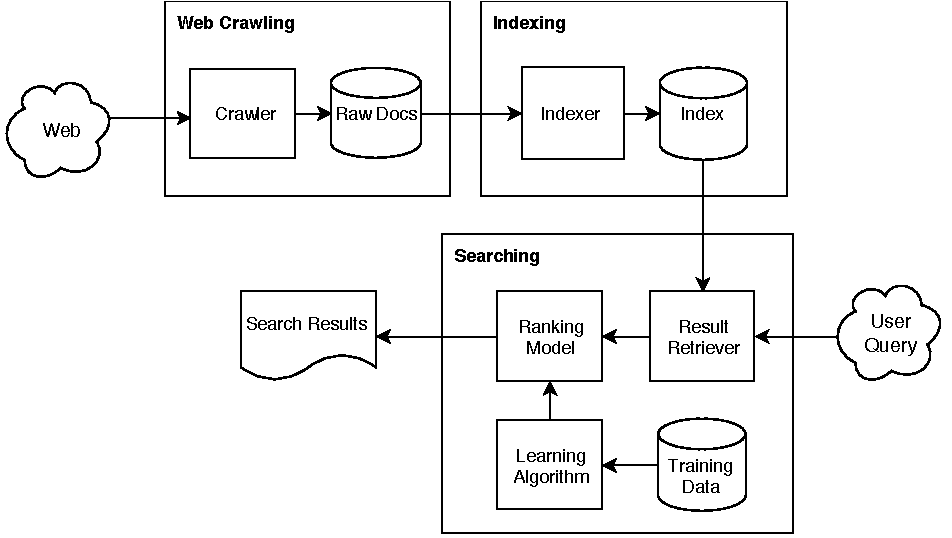
\includegraphics[width=0.8\textwidth]{img/searchengine.pdf}
  \caption{An example of a search engine architecture.}
  \label{fig:searchengine}
\end{figure}

Modern search engines use learning-to-rank algorithms for the ranking task. Learning to rank is the application of machine learning in information retrieval systems in order to construct ranking models. Such a model, typically supervised, is trained on training data consisting of query-document pairs, each with a relevance degree. The purpose of the model is to rank documents, i.e., produce an ordering that is optimal with respect to an evaluation metric.

Some of the evaluation metrics for ranking are mean average precision (MAP), discounted cumulative gain (DCG) and NDCG (normalized DCG), precision@n, NDCG@n (where @n denotes that the metrics are evaluated only on top n documents), mean reciprocal rank, Kendall's tau, and Spearman's rho. We use NDCG@n, so we will explain it in detail here. NDCG is a normalized version of discounted cumulative gain \citep{jarvelin2002cumulated}. Using a graded relevance scale of documents in a search-engine result set, DCG measures the usefulness, or gain, of a document based on its position in the result list. The gain is accumulated from the top of the result list to the bottom, with the gain of each result discounted at lower ranks. The graded relevance value is reduced logarithmically proportional to the position of the result, therefore penalizing highly relevant documents appearing lower in a search result list. The DCG at rank position $p$ is defined as:
\[ \mathrm {DCG_{p}} =\sum _{i=1}^{p}{\frac {rel_{i}}{\log _{2}(i+1)}}, \]
where $rel_{i}$ is the graded relevance of the result at position $i$.

We use normalized DCG, because search result lists vary in length depending on the query. In this case, the cumulative gain at each position for a chosen value of $p$ should be normalized across queries. We do this by sorting all relevant documents in the corpus by their relative relevance, producing the maximum possible DCG through position $p$, called Ideal DCG (IDCG) through that position. NDCG is defined as:
\[ \mathrm {nDCG_{p}} = \frac {\mathrm {DCG_{p}}}{\mathrm {IDCG_{p}}}, \]
and IDCG is defined as:
\[ \mathrm {IDCG_{p}} =\sum _{i=1}^{|REL|}{\frac {rel_{i}}{\log _{2}(i+1)}}, \]
where $|REL|$ represents the list of ordered relevant documents up to position $p$.

In an online scenario, when a user types a query into a search engine, they expect to see results in a very short time, typically a few hundred milliseconds. This makes it impossible to evaluate a complex ranking model, so modern search engines use a two-phase retrieval and ranking strategy \citep{cambazoglu2010early}. In the first phase, the scoring is very simple, enabling a quick retrieval process. Consequently, the second phase uses a more complex model, since now only a small subset of the overall document index is being ranked.

The query-document pairs are scored, then ranked, based on their feature vectors. The features can be divided into three groups:
\begin{enumerate}
	\item Query-independent or static features: features depending only on the document, but not on the query. For example, PageRank \citep{page1999pagerank} or the document's length. These features can be precomputed offline when indexing the document.
	\item Query-dependent or dynamic features: features depending both on the contents of the document and the query, such as the similarity between the query terms and the document content.
    \item Query features: features depending only on the query, such as the number of words in a query.
\end{enumerate}

\section{Problem Definition}
% talk about relevance vs recency and why it's difficult
The effectiveness of a search engine depends on the relevance of the result set it returns. Search engines employ ranking methods to provide the best results first. As more and more content is put on the Web, now more quickly than ever, the temporal aspect of results is very important for modern search engines. In web search, recency ranking refers to ranking the documents both by their relevance to the user query, and their freshness. The search engine can appear stale if it failed to recognize the temporal aspect of a query, which can also negatively affect the user experience. Effectively combining temporal features, as well as relevance-sensitive features in a ranking framework is still an open question for the research community.

The connection between relevance and recency is not always clear. In other words, if optimizing for only one of them, we might decrease the effectiveness of the search engine. Therefore, it is necessary to find an equilibrium. The trade-off can also depend on the user's query. For example, for a recency sensitive query, i.e., a query for which a user expects topically relevant documents to be also fresh, recency is very important. On the other hand, for timely queries, i.e., queries that do not show a spike in their popularity over time, relevance should be more important. Figure \ref{fig:serp} shows an example of a blend of relevant and recent results.

Even when the query type is identified, in order to incorporate both recent and relevant results, we need to determine the recency component on the document side. When dealing with general documents from the Web, this is not a trivial task, as most of the documents do not have any temporal information.

\begin{figure}
  \centering
  
\includegraphics[width=0.7\textwidth]{img/serp.png}
  \caption{An example of a search engine result page (SERP) from Google for the query \textit{Carles Puigdemont} submitted on June 29, 2018.}
  \label{fig:serp}
\end{figure}

In our experiments, we ask the following research questions:
\begin{enumerate}
    \item How can we determine if a document's content is recent without having information on its publication date?
    \item How can we determine when queries seek recent results?
    \item How can we introduce recency ranking into an existing relevance ranking architecture?
\end{enumerate}

\section{Contributions}
The contributions of this thesis are both theoretical and practical. In Chapter~\ref{ch:doc}, we present a document age prediction model, used to predict how recent a document is by extracting temporal evidence from its content. In Chapter \ref{ch:query}, we present a query recency sensitivity classifier, used to predict the need of recent results for a query. Finally, in Chapter \ref{ch:webranking}, we present a novel method of incorporating recency with the help of these two classifiers into an existing search engine. We also present an exhaustive evaluation of all presented models.
